The error propagation operator for a smoother is given by ${\color{burgundy}\mathbf{S}} = I - {\color{burgundy}\mathbf{M}}^{-1} {\color{burgundy}\mathbf{A}}$.

% -- Jacobi -------------------------------------------------------------------
\subsection{Jacobi}

Following the derivation from Section \ref{sec:lfahighorder}, the symbol of the Jacobi error propagation operator is given by
\begin{equation}
\tilde{{\color{burgundy}\mathbf{S}}} \left( \omega, \theta \right) = I - \tilde{{\color{burgundy}\mathbf{M}}}^{-1} \left( \theta \right) \tilde{{\color{burgundy}\mathbf{A}}} \left( \theta \right) = I - \left( \mathbf{Q}^T \diag \left( {\color{burgundy}\mathbf{A}}_e \right)^{-1} \mathbf{Q} \right) \tilde{{\color{burgundy}\mathbf{A}}} \left( \theta \right),
\end{equation}
where this expression has been simplified by the fact that $e^{\imath \left( x_i - x_i \right) \theta / h} = 1$.

\begin{definition}
The symbol of the error propagation operator for Jacobi smoothing is given by
\begin{equation}
\tilde{{\color{burgundy}\mathbf{S}}} \left( \nu, \omega, \theta \right) = \left( I - \left( \mathbf{Q}^T \diag \left( {\color{burgundy}\mathbf{A}}_e \right)^{-1} \mathbf{Q} \right) \tilde{{\color{burgundy}\mathbf{A}}} \left( \theta \right) \right)^\nu,
\end{equation}
where $\nu$ is the number of smoothing passes.
\label{def:jacobi_symbol}
\end{definition}

\begin{figure}[!tbp]
  \centering
  \subfloat[Spectrum of Jacobi for $p = 4$]{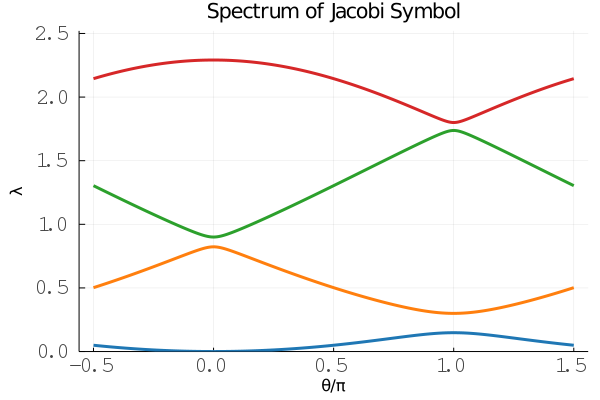
\includegraphics[width=0.48\textwidth]{images/jacobi_spectrum_5}\label{fig:jacobi_spectrum}}
  \hfill
  \subfloat[Smoothing Factor of Jacobi for $p = 4$]{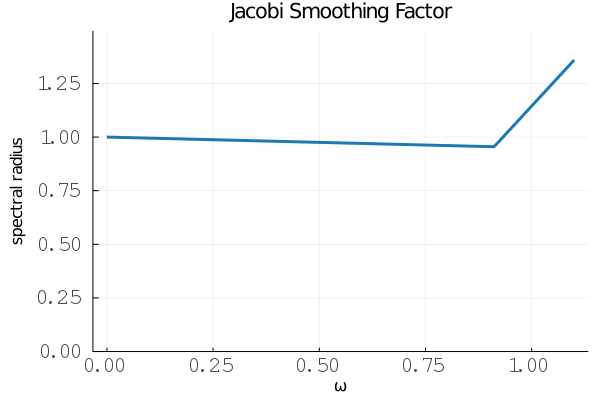
\includegraphics[width=0.48\textwidth]{images/jacobi_smoothing_5}\label{fig:jacobi_smooth_factor}}
  \caption{Jacobi smoothing for high-order finite elements}
\end{figure}

Using Definition \ref{def:jacobi_symbol}, we plot the eigenvalues of $\tilde{{\color{burgundy}\mathbf{M}}}^{-1} \tilde{{\color{burgundy}\mathbf{A}}} \left( \theta \right)$ in Figure \ref{fig:jacobi_spectrum} for the one dimensional Laplacian with a 4th order basis on Gauss-Lobatto points.
In Figure \ref{fig:jacobi_smooth_factor} we plot the LFA smoothing factor for Jacobi smoothing as a function of the smoothing parameter $\omega$.

% -- Chebyshev ----------------------------------------------------------------
\subsection{Chebyshev}

It is well known that polynomial smoothers allow more aggressive coarsening than Jacobi \cite{brannick2015polynomial};
however, for this analysis we use a simple Jacobi smoother, with $M = \diag \left( A \right)$.
